\section{Conjugate-closed grids}\label{sec:conj}

The two uncolorable grids of $\{0,\pm1,\pm\sqrt2\}$ and $\{0,\pm1,\pm\sqrt{-2}\}$ both have
$|x|^2=2$, and in both the conjugate $x^{*}=\pm x$ is already a coordinate value.  For a general
complex $x$ the list of coordinate values that is closed under conjugation is
\[
\mathcal A(x)=\{0,\pm1,\pm x,\pm x^{*}\},\qquad P(x)=S(\mathcal A(x)).
\]
For generic $x$ the grid $P(x)$ has 145 rays; at special $x$ some of them coincide (49 remain
at $x=\sqrt{\pm2}$).  This section determines every $x$ at which $P(x)$ is uncolorable
(Theorem~\ref{thm:conj}, Fig.~\ref{fig:circle}): two circles, four lines through the origin
with the origin removed, and four points.  It
then takes the two circles in turn.  On $|x|^2=2$ one fixed list of 45 coordinate triples is uncolorable at
every point (Theorem~\ref{thm:circle}).  On $|x|^2=\tfrac12$ the grid contains the 33-ray family
of Gould and Aravind (Section~\ref{sec:halfcircle}).

\begin{figure}[t]
\centering
\begin{tikzpicture}[scale=1.55]
\draw[->,gray] (-2.45,0) -- (2.6,0) node[right] {$\mathrm{Re}\,x$};
\draw[->,gray] (0,-2.1) -- (0,2.25) node[above] {$\mathrm{Im}\,x$};
\foreach \t in {30,60,120,150} \draw[line width=0.9pt] (\t:-1.9) -- (\t:1.9);
\draw[line width=0.9pt] (0,0) circle (1.4142);
\draw[line width=0.9pt] (0,0) circle (0.7071);
\foreach \p in {-2,-0.5,0.5,2} \fill (\p,0) circle (0.05);
\draw[fill=white,line width=0.5pt] (0,0) circle (0.06);
\node[font=\small,anchor=south west] at (2.0,0.06) {\textit{B}\ \,$2$: $\CK$};
\fill (1.4142,0) circle (0.05) node[below right,font=\small] {\textit{A}\ \,$\sqrt2$: Peres};
\draw[fill=white,line width=0.5pt] (1.7321,0) circle (0.05);
\node[font=\small,anchor=south] at (1.7321,0.06) {\textit{C}};
\fill (0,1.4142) circle (0.05);
\node[font=\small,anchor=south west] at (0.08,1.78) {$\sqrt{-2}$: 33 rays};
\draw[gray,line width=0.3pt] (0.03,1.46) -- (0.12,1.8);
\fill (0.5,1.3229) circle (0.05);
\node[font=\small,anchor=west] at (1.2,1.45) {$\tfrac{1+\sqrt{-7}}{2}$: minimum 43};
\draw[gray,line width=0.3pt] (0.55,1.34) -- (1.18,1.44);
\node[font=\small,anchor=east] at (-1.25,1.5) {$|x|^2=2$};
\node[font=\small,anchor=east] at (-1.75,-0.5) {$|x|^2=\tfrac12$};
\draw[gray,line width=0.3pt] (-0.69,-0.17) -- (-1.73,-0.48);
\node[font=\small,anchor=west] at (1.68,-0.97) {$\arg x=-30^\circ$};
\node[font=\small,anchor=north west] at (0.97,-1.66) {$\arg x=-60^\circ$};
\node[font=\small,align=left,anchor=north east] at (-1.2,-1.5) {elsewhere:\\colorable};
\end{tikzpicture}
\caption{The grid with coordinate values $\{0,\pm1,\pm x,\pm x^{*}\}$.  It is uncolorable exactly on the set
drawn in black: the circles $|x|^2=2$ and $|x|^2=\tfrac12$, the four lines through the origin at
$\pm30^\circ$ and $\pm60^\circ$ to the real axis with the origin removed, and the points
$\pm2,\pm\tfrac12$ (Theorem~\ref{thm:conj}).  The grid is unchanged by $x\mapsto-x$ and
$x\mapsto x^{*}$, so one quadrant suffices.  At the four axis points of the outer circle, which
are two grids up to sign, the 45 coordinate triples of Table~\ref{tab:words} collapse to 33 rays.  At $(1+\sqrt{-7})/2$ the additional
relation $x+x^{*}=1$ adds orthogonalities and the minimum drops from 45 to~43.
\textit{A}, \textit{B} and \textit{C} are the three cubes of Fig.~\ref{fig:triptych}, left to
right.  At these three real values $x^{*}=x$ and $P(x)$ is the 49-ray grid of
Section~\ref{sec:real}; \textit{C} is $x=\sqrt3$ (open circle), where the grid has a coloring.}
\label{fig:circle}
\end{figure}

\subsection{The classification}\label{sec:conjclosed}

\begin{theorem}[Conjugate-closed grids]\label{thm:conj}
Let $x$ be a nonzero complex number and $P(x)$ the grid with coordinate values
$\{0,\pm1,\pm x,\pm x^{*}\}$.
\begin{enumerate}[label=(\roman*)]
\item $P(x)$ is uncolorable if and only if one of the following holds:
\begin{enumerate}[label=(\alph*)]
\item $|x|^2=2$;
\item $|x|^2=\tfrac12$;
\item $x^{*}/x$ is a primitive third or sixth root of unity, that is, $\arg x$ is one of
$\pm30^\circ$, $\pm60^\circ$, $\pm120^\circ$, $\pm150^\circ$;
\item $x\in\{\pm2,\pm\tfrac12\}$.
\end{enumerate}
\item At every point of the curves (a)--(c) other than the special points of
Table~\ref{tab:conj}, the minimum uncolorable subset of $P(x)$ has 45 rays on $|x|^2=2$ and 33
rays on $|x|^2=\tfrac12$ and on the four lines of~(c).  At the special points the minima are
those of Table~\ref{tab:conj}; two of them are bounds and not certified values.
\item For every $x$ other than $\pm1\pm i$, no uncolorable subset of $P(x)$ has fewer than 31
rays, and 31 is attained at $x=\pm2,\pm\tfrac12$, where $P(x)$ is the integer grid.  At
$x=\pm1\pm i$ the grid is uncolorable and we have not established the bound 31; there the
minimum lies between the general lower bound 24 and~45.
\end{enumerate}
\end{theorem}

\begin{proof}
The argument is that of Theorem~\ref{thm:twosymbol} with two more monomials.  An inner product of
two coordinate triples, and a $2\times2$ minor of two coordinate triples, is an integer combination
\[
c_0+c_1x+c_2x^{*}+c_3|x|^2+c_4x^2+c_5x^{*2}
\]
with $\sum|c_k|\le3$; 376 nonzero coefficient vectors occur.  With $x=a+ib$ the combination
vanishes when
\[
b\,\bigl[(c_1-c_2)+2(c_4-c_5)\,a\bigr]=0,\qquad
c_0+(c_1+c_2)\,a+(c_3+c_4+c_5)\,a^2+(c_3-c_4-c_5)\,b^2=0 .
\]
Both conditions involve $b$ only through the factor $b$ and through $b^2$, and the second is
linear in~$b^2$.  The solution set of one vector is therefore made up of finitely many points
and of whole curves of three kinds: the real axis, a vertical line, and a curve
$b^2=g_0+g_1a+g_2a^2$.  We work throughout in the coordinates $(a,b^2)$, which identifies $x$
with $x^{*}$; this loses nothing, because $P(x^{*})=P(x)$.  Two different curves of these kinds
meet in at most two values of~$a$.  A vector that vanishes at infinitely many points of a curve
$b^2=g(a)$ with $b\ne0$ vanishes on all of it: the first condition then forces
$(c_1-c_2)+2(c_4-c_5)a$ to be identically zero, and substituting $b^2=g(a)$ in the second
gives a polynomial in $a$ with infinitely many roots.  So the two lines of a pair such as
$b^2=3a^2$, and the two branches of a hyperbola, need not be treated separately.
Going through the 376 vectors gives fourteen curves with points other than the origin:
\[
\mathrm{Im}\,x=0,\quad \mathrm{Re}\,x=0,\ \pm\tfrac12,\quad |x|^2=\tfrac12,\ 1,\ 2,\quad
|x\pm1|=1,\quad \mathrm{Re}\,x^2=0,\ \pm\tfrac12,\quad x^2+x^{*2}=\pm|x|^2 .
\]
The last two are the pairs of lines $b^2=a^2/3$ and $b^2=3a^2$ of part~(c).  Call a nonzero point
\emph{special} if it is an isolated solution of some vector or lies on two of the curves; there
are 53 special points with $\mathrm{Im}\,x\ge0$ (92 in the plane, 14 of them real).  As in Theorem~\ref{thm:twosymbol}, the set of vectors that vanish at $x$,
and with it the list of proportional coordinate triples and the orthogonality graph of $P(x)$, is the same at
all points on no curve, and the same at all non-special points of any one curve.  That leaves
$1+14+53=68$ cases.  The grid is also unchanged by $x\mapsto-x$, which reduces
the special points to 28 classes and the curves to 12; unlike the grid with two coordinate values it is not
unchanged by $x\mapsto1/x$.

The script \texttt{ks\_conjugate\_closed\_theorem.py} lists the curves and the special points in
exact arithmetic ($a$ and $b^2$ in one quadratic field $\Q(\sqrt d)$), builds the 68 graphs, decides colorability of
each, and runs the certification procedure of Section~\ref{sec:methods} on the uncolorable ones.
Table~\ref{tab:conj} is the result.  The uncolorable cases are the curves (a), (b) and (c), every
special point on them, and the points $\pm2,\pm\tfrac12$; all other cases are colorable.  That
is~(i).  Part~(ii) is the corresponding rows of the table.  For~(iii), the certifier terminated
with a minimum of at least 31 in every uncolorable case except four.  For those four we made
separate runs, each of which only decides whether an uncolorable subset of fewer than a given
number of rays exists.  At $\eta/\sqrt2$ and at $2\zeta$
(notation of Table~\ref{tab:conj}) there is none of fewer than 33 rays,
which with the 33-ray sets found makes 33 the minimum.  At $\zeta/\sqrt2$ there is none of
fewer than 32, and the run for 33 did not terminate in eight hours.  At $x=\pm1\pm i$ the run
for 31 did not terminate in eight hours.  The
witnesses are archived; the lists of colorable sets produced by these runs are not, so the
lower bounds of this theorem can be reproduced only by rerunning the script.

Part~(c) also has a proof that needs no new computation.  A coordinate triple whose nonzero entries are all
$\pm x$ or $\pm x^{*}$ is $x$ times a coordinate triple of $\{0,\pm1,\pm u\}$ with $u=x^{*}/x$, so $P(x)$
contains every ray of the grid $S(u)$.  By Theorem~\ref{thm:twosymbol}, $S(u)$ is
uncolorable when $u$ is a primitive third or sixth root of unity, with a 33-ray minimum set
having the graph of the Eisenstein set, and Lemma~\ref{lem:restrict} carries this to $P(x)$.
This argument gives nothing more, since $S(u)$ is colorable for every other $u$ on the unit
circle.
\end{proof}

\begin{table}[t]
\centering
\caption{Every conjugate-closed grid, coordinate values $\{0,\pm1,\pm x,\pm x^{*}\}$
(Theorem~\ref{thm:conj}).  A curve stands for its points other than the special points listed
below it, and each special point stands for its images under $x\mapsto-x$ and
$x\mapsto x^{*}$.  $\zeta=e^{i\pi/3}$, $\eta=e^{i\pi/6}$, $\varphi=(1+\sqrt5)/2$.  ``Min'' is
the certified size of the smallest uncolorable subset; ``32--33'' means that 33 rays suffice
and fewer than 32 do not; ``$\le45$'' is an upper bound only.  The last column gives the graph
of the smallest set found (isomorphism by VF2).}
\label{tab:conj}
\small
\begin{tabular}{@{}lrrrcl@{}}
\toprule
$x$ & Rays & Pairs & Triads & Min & Smallest set found \\
\midrule
on no curve & 145 & 366 & 22 & --- & colorable \\
$\mathrm{Im}\,x=0$;\ \ $\mathrm{Re}\,x=0$ & 49 & 114 & 10 & --- & colorable \\
$|x|=1$ & 109 & 276 & 16 & --- & colorable \\
$\mathrm{Re}\,x^2=0$ & 127 & 321 & 19 & --- & colorable \\
$\mathrm{Re}\,x=\pm\tfrac12$;\ \ $|x\pm1|=1$ & 145 & 462 & 30 & --- & colorable \\
$\mathrm{Re}\,x^2=\pm\tfrac12$ & 145 & 378 & 22 & --- & colorable \\
$|x|^2=2$ & 145 & 378 & 34 & \textbf{45} & 45 rays, 98 pairs \\
$|x|^2=\tfrac12$ & 145 & 390 & 46 & \textbf{33} & Peres \\
$\arg x=\pm30^\circ,\pm60^\circ,\pm120^\circ,\pm150^\circ$ & 145 & 390 & 30 & \textbf{33} & Eisenstein 33 \\
\midrule
$1$ & 13 & 24 & 4 & --- & colorable \\
$i$ & 31 & 69 & 7 & --- & colorable \\
$\varphi,\ 1/\varphi$ & 49 & 138 & 10 & --- & colorable \\
$e^{i\pi/4}$ & 91 & 231 & 13 & --- & colorable \\
$|x-1|=1$ and $\mathrm{Re}\,x^2=\tfrac12$ & 145 & 474 & 30 & --- & colorable \\
\midrule
$2,\ \tfrac12$ & 49 & 138 & 26 & \textbf{31} & $\CK$ \\
$\sqrt2,\ 1/\sqrt2,\ \sqrt{-2},\ 1/\sqrt{-2}$ & 49 & 120 & 16 & \textbf{33} & Peres \\
$(1+i)/2$ & 127 & 465 & 51 & \textbf{33} & Peres \\
$(1+\sqrt{-7})/4$ & 145 & 486 & 54 & \textbf{33} & Peres \\
$\eta/\sqrt2$ & 145 & 414 & 54 & \textbf{33} & Peres \\
$\zeta/\sqrt2$ & 145 & 414 & 54 & 32--33 & Peres \\
$\zeta$ & 57 & 174 & 22 & \textbf{33} & Eisenstein 33 \\
$\eta$ & 109 & 312 & 24 & \textbf{33} & Eisenstein 33 \\
$\zeta/2$ & 145 & 414 & 54 & \textbf{33} & Eisenstein 33 \\
$\eta/\sqrt3,\ \sqrt3\,\eta$ & 145 & 486 & 38 & \textbf{33} & Eisenstein 33 \\
$\sqrt2\,\eta,\ \sqrt2\,\zeta$ & 145 & 402 & 42 & \textbf{33} & Eisenstein 33 \\
$2\zeta$ & 145 & 438 & 62 & \textbf{33} & Eisenstein 33 \\
$(1+\sqrt{-7})/2$ & 145 & 522 & 42 & \textbf{43} & 43 rays, 107 pairs \\
$(\sqrt5+\sqrt{-3})/2,\ (\sqrt3+\sqrt{-5})/2$ & 145 & 390 & 34 & \textbf{45} & 45 rays, 98 pairs \\
$1+i$ & 127 & 477 & 63 & $\le45$ & 45 rays, 98 pairs \\
\bottomrule
\end{tabular}
\end{table}

Five remarks.

First, the theorem says where $P(x)$ is uncolorable and not why.  For the circle $|x|^2=2$,
Section~\ref{sec:circle} gives a reason: a fixed list of 45 coordinate triples whose orthogonalities follow
from $xx^{*}=2$ alone (Theorem~\ref{thm:circle}).  Part~(ii) of that theorem says that $P(x)$ is
colorable outside a finite union of proper real algebraic subsets; the present theorem
identifies the union as two circles, four lines without the origin, and four points.

Second, the three curves behave differently.  On $|x|^2=2$ the minimum is 45 except at
finitely many points.  On $|x|^2=\tfrac12$ it is 33 except possibly at the one class of
points marked 32--33, and the smallest set found has the orthogonality graph of Peres's set at
a generic point and at every special point of that circle (Section~\ref{sec:halfcircle}).
Every point of the lines other than the origin has a
33-ray uncolorable set with the graph of the Eisenstein set of Section~\ref{sec:roots}, written
in the coordinate values $\{0,\pm x,\pm x^{*}\}$, by the last paragraph of the proof; it is a minimum set
wherever the table certifies~33.

Third, earlier versions surveyed the grids of $\{0,\pm1,\pm a,\pm a^{*}\}$ with $a$ the
generator of the ring of integers of $\Q(\sqrt{-d})$, for the nine imaginary quadratic fields
of class number one, and looked for an arithmetic reason why $d=2,3,7$ give uncolorable grids.
The theorem accounts for the survey without reference to number fields: $d=2$ and $d=7$ are
points of $|x|^2=2$; $d=3$ is the point $\zeta$ of the $60^\circ$ line; $d=1$ is $x=i$,
colorable; and for $d=11,19,43,67,163$ the generator lies on $\mathrm{Re}\,x=\tfrac12$ and on no
uncolorable curve (145 rays, 462 pairs, 30 triads, as in the table).  The row $(1+i)/2$ of
Table~\ref{tab:conj} is the Gaussian grid, with coordinate values $\{0,\pm1,\pm i,\pm(1+i)\}$, of
Table~\ref{tab:catalogue}, after multiplying every coordinate value by $1+i$.

Fourth, the certified minima of Table~\ref{tab:conj} are 31, 33, 43 and 45.  The grid with
the conjugate does not give a KS set smaller than that of Conway and Kochen at any point where
the computation finished, and among the certified cases 31 is reached only by the integer grid.
The statement is incomplete at $x=\pm1\pm i$, where the certifier did not terminate, and at the
class marked 32--33, where the minimum is 32 or 33.

Fifth, like Theorem~\ref{thm:twosymbol} this concerns grids.  Completed grids are not
covered.

The script asserts agreement with the number-field constructions of
Section~\ref{sec:catalogue} at seven points, at a generic point and on the circle $|x|^2=2$;
we also rebuilt six further cases with those constructions and found the same counts.  The
graphs of the smallest sets are identified by \texttt{ks\_conjugate\_closed\_identify.py}.

\subsection{The circle $|x|^2=2$}\label{sec:circle}

Earlier versions of this paper met the conjugate-closed grid at one point,
$x=(1+\sqrt{-7})/2$, found it uncolorable, and attributed that to the arithmetic of the
ring of integers of $\Q(\sqrt{-7})$.  It is a property of the whole circle, and it has a proof
that does not go through the case analysis of Theorem~\ref{thm:conj}.

\begin{theorem}\label{thm:circle}
Let $W$ be the list of 45 coordinate triples in Table~\ref{tab:words}, expressions in $x$ and $x^{*}$.
\begin{enumerate}
\item[(i)] For every $x\in\C$ with $|x|^2=2$ the rays of $W$ form a KS-uncolorable set.
Consequently $P(x)$ is uncolorable for every such~$x$.
\item[(ii)] The orthogonalities among 145 coordinate triples, one naming each ray of $P(x)$ at generic~$x$, that hold for every
$x\in\C$ form a colorable
configuration (366 pairs, 22 triads).  Hence $P(x)$ is colorable for every $x$ outside a finite
union of proper real algebraic subsets of~$\C$.
\item[(iii)] No list of fewer than 45 of the 145 coordinate triples is uncolorable by virtue of the
orthogonalities that hold along the whole circle.  Consequently no fixed list of fewer than 45
coordinate triples with coordinate values $\mathcal A(x)$ is uncolorable at every point of the circle.
\end{enumerate}
Part~(iii) concerns fixed lists of coordinate triples of this grid.  It says nothing about other
parametrized families of KS sets.
\end{theorem}

\begin{proof}
The inner product of two coordinate triples is a polynomial in $x$ and $x^{*}$ with integer coefficients, of
degree at most~2.

(i)  On the circle, $xx^{*}=2$ reduces every such polynomial to an integer combination of
$1,x,x^{*},x^2,x^{*2}$.  With $x=\sqrt2e^{i\theta}$ these are constant multiples of
$e^{ik\theta}$, $k=0,\pm1,\pm2$, which are linearly independent functions of~$\theta$.  So an
inner product vanishes at every point of the circle if and only if every reduced coefficient is
zero, a finite check in integers.  It yields 98 pairs among the coordinate triples of $W$ that are orthogonal
at every point of the circle, forming the 22 triads listed in Appendix~\ref{app:triads}.  A SAT
solver shows that the configuration with these 98 exclusions and 22 triads has no coloring.  Now
fix $x$ on the circle.  If the 45 coordinate triples give 45 distinct rays, the orthogonality graph at $x$
contains the 98 pairs, and any further pairs or triads only add constraints, so there is no
coloring.  If two coordinate triples give the same ray, a coloring at $x$ assigns them the same value and so
would also be a coloring of the 45-vertex configuration; there is none.  (Two coordinate triples that are
orthogonal for every $x$ on the circle cannot coincide at any point of it.)

(ii)  Without the relation, the monomials $x^ax^{*b}$ are linearly independent functions
on~$\C$, so an inner product vanishes for all $x$ iff all its coefficients vanish.  This yields
366 pairs and 22 triads on the 145 coordinate triples, and a SAT solver finds a coloring.  Each remaining
inner product is a nonzero polynomial in $x,x^{*}$ and vanishes only on a proper real algebraic
subset.  For each pair of the 145 coordinate triples at least one $2\times2$ minor of the pair is a nonzero
polynomial, so the set of $x$ at which the two coordinate triples give the same ray is also a proper real
algebraic subset.  Away from those finitely many subsets the 145 rays are distinct, no further
pair is orthogonal, and the coloring found is a coloring of $P(x)$.

(iii)  The 145 coordinate triples with the pairs and triads that hold along the whole circle (378 pairs, 34
triads) form a finite configuration, and the certifier of Section~\ref{sec:methods} returns 45 as
its minimum, with a certificate of 408 colorable sets.  For the consequence: the exceptional
points of the circle, at which some further inner product vanishes or two coordinate triples name the same ray, are
finite in number, since each such condition is a nonzero trigonometric polynomial in~$\theta$.
A list uncolorable at every point of the circle is uncolorable at a non-exceptional point, where
the configuration is exactly the one just described.

The script \texttt{ks\_modulus2\_circle.py} carries out all three computations.  Its
output file, \texttt{results/modulus2\_circle.json}, holds the 145 coordinate triples, both graphs, the
coloring of part~(ii) and the certificate of part~(iii).
\end{proof}

Part~(i) is also proved in Lean~4: for every complex $x$ with $xx^{*}=2$, the 45 coordinate triples admit
no coloring (theorem \texttt{Circle45.uncolorable} in the file \texttt{NamedSets.lean}).  The Lean proof follows the argument above.  Inner products are reduced with
$xx^{*}=2$ and nothing else, so every orthogonality it uses holds at every point of the circle;
the orthogonal pairs are recomputed inside Lean; and a case-split refutation of every coloring
is checked by the kernel.  Parts (ii) and~(iii) are not formalized.

\begin{table}[t]
\centering
\caption{The 45 coordinate triples of Theorem~\ref{thm:circle}.  A bar is a minus sign and $x^{*}$ is the
complex conjugate, so $\bar x^{*}=-x^{*}$.  The list is one minimum set; we have not enumerated
the others.}
\label{tab:words}
\small
\begin{tabular}{rl@{\qquad}rl@{\qquad}rl@{\qquad}rl@{\qquad}rl}
\hline
1 & $0\,0\,1$ & 10 & $1\,0\,1$ & 19 & $1\,1\,x^{*}$ & 28 & $1\,x^{*}\,\bar 1$ & 37 & $x\,\bar 1\,0$ \\
2 & $0\,1\,0$ & 11 & $1\,0\,\bar 1$ & 20 & $1\,1\,\bar x^{*}$ & 29 & $1\,\bar x^{*}\,0$ & 38 & $x\,\bar 1\,1$ \\
3 & $0\,1\,1$ & 12 & $1\,0\,x$ & 21 & $1\,\bar 1\,0$ & 30 & $1\,\bar x^{*}\,1$ & 39 & $x\,\bar 1\,\bar 1$ \\
4 & $0\,1\,\bar 1$ & 13 & $1\,0\,\bar x$ & 22 & $1\,\bar 1\,x$ & 31 & $1\,\bar x^{*}\,\bar 1$ & 40 & $x^{*}\,0\,1$ \\
5 & $0\,1\,x$ & 14 & $1\,0\,x^{*}$ & 23 & $1\,\bar 1\,\bar x$ & 32 & $x\,0\,1$ & 41 & $x^{*}\,0\,\bar 1$ \\
6 & $0\,1\,\bar x$ & 15 & $1\,0\,\bar x^{*}$ & 24 & $1\,\bar 1\,x^{*}$ & 33 & $x\,0\,\bar 1$ & 42 & $x^{*}\,1\,1$ \\
7 & $0\,x^{*}\,1$ & 16 & $1\,1\,0$ & 25 & $1\,\bar 1\,\bar x^{*}$ & 34 & $x\,1\,0$ & 43 & $x^{*}\,1\,\bar 1$ \\
8 & $0\,x^{*}\,\bar 1$ & 17 & $1\,1\,x$ & 26 & $1\,x^{*}\,0$ & 35 & $x\,1\,1$ & 44 & $x^{*}\,\bar 1\,1$ \\
9 & $1\,0\,0$ & 18 & $1\,1\,\bar x$ & 27 & $1\,x^{*}\,1$ & 36 & $x\,1\,\bar 1$ & 45 & $x^{*}\,\bar 1\,\bar 1$ \\
\hline
\end{tabular}

\end{table}

Comparing (i) and (ii): of the 378 pairs present along the circle, 366 are present for every
$x$, and the other 12 are all of the form $1+1-x^{*}x=0$, as in
$(x,1,1)\perp(x,\bar1,\bar1)$.  With them come 12 further triads.  These 12 pairs are the
difference between a colorable grid and an uncolorable one, and the relation behind them is the
one Peres's cube uses at $x=\sqrt2$ (Fig.~\ref{fig:generic}).

\begin{corollary}\label{cor:points}
\begin{enumerate}
\item[(a)] At $x=\sqrt2$ and at $x=\sqrt{-2}$ the 45 coordinate triples give exactly 33 distinct rays.  By
Computed fact~\ref{fact:peres} these are the unique minimum sets of those grids; at $x=\sqrt2$
they are the 33 rays of Peres.
\item[(b)] At $x=(1+\sqrt{-7})/2$, $P(x)$ is the 145-ray grid studied in earlier versions.  It is
uncolorable because $|x|^2=2$.
\item[(c)] The coordinate triples $(1,1,x)$ and $(1,0,x^{*})$ of $W$ have squared overlap
$|1+x^{*2}|^2/12=(5+4\cos2\theta)/12$, which is not constant.  The sets of part~(i) are therefore
not all unitarily equivalent: the multiset of squared overlaps between rays is a unitary
invariant that does not depend on labelling, and it takes infinitely many values along the
circle.
\item[(d)] At $x=(1+\sqrt{-7})/2$ the 45 coordinate triples give 45 distinct rays with 114 orthogonal pairs
and 26 triads, and this set contains a 43-ray KS subset; 43 is the certified minimum within it.
\end{enumerate}
\end{corollary}

\subsection{The point $x=(1+\sqrt{-7})/2$}

Let $\alpha=(1+\sqrt{-7})/2$, so $|\alpha|^2=2$ and $\alpha+\alpha^{*}=1$.

\begin{fact}[The $\Q(\sqrt{-7})$ grid]\label{fact:heegner}
$P(\alpha)$ has 145 rays, 522 orthogonal pairs and 42 triads, against 378 and 34 at a generic
point of the circle.  Its minimum uncolorable subsets have 43 rays, certified.  There are exactly
six of them, in two orbits under signed permutations of the coordinates, each with 23 bases; the
one we use has 107 pairs and degree sequence $4^{16}5^{20}6^{4}8^{2}10^{1}$.  The completed grid
has 685 rays, 1746 pairs and 582 triads; its minimum is \heegnercompletedmin.
\end{fact}

So the additional relation at this point is worth two rays: 43 against 45
(Corollary~\ref{cor:points}d).  It is the grids $P(x)$ that form a continuous family through
this point.  Theorem~\ref{thm:circle} proves that $P(\alpha)$ is uncolorable; that its minimum is
43 is a separate computation.  Both halves of that minimum are also proved in Lean
(\texttt{KSMin.HeegnerPool.minimum\_43}, Section~\ref{sec:methods}): some 43 of the 145 rays are
uncolorable, and every set of fewer than 43 of them is colorable.

\subsection{The circle $|x|^2=\tfrac12$: the family of Gould and Aravind}\label{sec:halfcircle}

On $|x|^2=\tfrac12$ the smallest uncolorable set found has 33 rays and the orthogonality graph
of Peres's set, at a generic point and at every special point (Table~\ref{tab:conj}).  So this
circle carries a one-parameter family of 33-ray sets with Peres's graph, joining Peres's set
($x=1/\sqrt2$) to the $\sqrt{-2}$ set ($x=i/\sqrt2$).  It is the family of Gould and
Aravind~\cite{GouldAravind2010}, who exhibited 33-ray sets with the graph of Peres's set,
depending on three phases and containing the sets of Peres and of Penrose; Flores
Gordillo~\cite{FloresGordillo2026} reports that after removing diagonal unitaries their family
is a circle.  The following are exact symbolic computations
(\texttt{ks\_half\_circle\_family.py exact}), writing $x=e^{i\theta}/\sqrt2$.
\begin{enumerate}[label=(\alph*)]
\item Exactly 72 inner products of the 33 coordinate triples vanish identically in~$x$, no other inner
product vanishes anywhere on the circle, and no two coordinate triples become proportional.  So the graph is
Peres's along the whole circle, not only at the special points.
\item Substituting $a=b=1$ and $c=1/x^{*}$ in Table~3 of Ref.~\cite{GouldAravind2010} gives our
33 coordinate triples, ray for ray; and for general $a,b$ (of modulus~1) the diagonal unitary
$\mathrm{diag}(b,a,1)$ carries their set with parameters $(a,b,c)$ to their set with parameters
$(1,1,ab^{*}c)$.  So up to unitary equivalence their three-parameter family is our circle, in
agreement with Flores Gordillo's reduction.
\item The maps $x\mapsto-x$ and $x\mapsto x^{*}$ (the latter followed by exchanging the first
two coordinates) carry the set of 33 rays to itself, so the members at $\theta$, $\theta+\pi$
and $-\theta$ are unitarily equivalent.
\item For unit vectors, $\sum_{i<j}|\braket{v_i}{v_j}|^4=
\tfrac{37493}{432}+\tfrac{17}{2}\cos2\theta$, which is strictly decreasing on $[0,\pi/2]$.
Hence the members with $0\le\theta\le\pi/2$ are pairwise unitarily inequivalent, and every
member is equivalent to one of them.
\end{enumerate}
Gould and Aravind identify Penrose's 33 rays with the parameters
$a=-i$, $b=-1$, $c=-\sqrt2$, which we have not re-derived.  These give $x=-i/\sqrt2$, so on that
identification Penrose's set is unitarily equivalent to the $\sqrt{-2}$ set; consistently, the
overlap of rays 9 and~14 is $(2-\sqrt2)/4$ at $\theta=0$ and $\sqrt6/4$ at $\theta=\pi/2$, the
values they give for Peres's and Penrose's sets.

This family is different from the one in Theorem~\ref{thm:circle}.  Its members have 33 rays
and a constant graph.  The family of Theorem~\ref{thm:circle} has 45 rays at a generic point and
cannot contain a 33-ray KS set there, since the minimum at a generic point of that circle is 45
(Theorem~\ref{thm:conj}).  The two families meet in Peres's set: $P(\sqrt2)=P(1/\sqrt2)$, a
49-ray grid whose unique minimum subset is Peres's set.  We
have not found the family of Theorem~\ref{thm:circle} in the literature, but we have not made a
systematic search and make no claim of priority.

\subsection{Rigidity}\label{sec:rigidity}

For the minimum sets and uncolorable witnesses named below we computed numerically the number
of infinitesimal flexes in $\C^3$: the
dimension of the null space of the Jacobian of the equations $|v_i|^2=1$,
$\braket{v_i}{v_j}=0$ (one complex equation for each orthogonal pair), minus the $n+8$
dimensions accounted for by a common unitary and a phase on each vector.  In every case the
smallest retained singular value exceeds $0.2$ and the largest discarded one is below
$2\times10^{-15}$.  The counts (\texttt{ks\_rigidity\_v10.py}, and
\texttt{ks\_half\_circle\_family.py} for the family on $|x|^2=\tfrac12$) are: no flex for $\CK$,
the Eisenstein 33-ray set, the 43-ray set, the two 47-ray supergolden sets (the minimum set of
the grid with three coordinate values, and the witness in the completed grid of $\{0,\pm1,\pm\psi\}$), the
51- and 60-ray witnesses of Section~\ref{sec:catalogue}, which are not known to be minimum sets,
and the 45 coordinate triples at $x=(1+\sqrt{-7})/2$ with the 16 additional
orthogonalities of that point imposed; one flex for the Peres and $\sqrt{-2}$ sets and for each
of nine sampled members of the family on $|x|^2=\tfrac12$; two flexes for the 45 coordinate triples at each
of the two generic phases tried ($\theta=0.3$ and $\theta=1.0$).  Zero flexes, if confirmed by
an exact rank computation, means the set is locally rigid.  It does not by itself mean that the
realization is unique up to unitary equivalence; for $\CK$ that stronger statement is the
theorem of Trandafir and Cabello~\cite{TrandafirCabello2025}, and for the Eisenstein set it is
asserted by Cabello~\cite{Cabello2025simplest}.  The single flex of the Peres set is the circle
of Section~\ref{sec:halfcircle}, a genuine deformation and not merely an infinitesimal one.
(Versions 1--7 claimed the opposite on the strength of a second-order computation with an
indexing error, found by Flores Gordillo and corrected in version~8.)  Of the two flexes of the
45 coordinate triples, one is motion along the circle (Corollary~\ref{cor:points}c); we have not identified
the other.
